\section{Shallow Safety Alignment is Not Durable to Downstream Fine-tuning}
\label{sec:fine-tuning-safety-improvement}

The central position of this paper is that many of the vulnerability problems, from which the current safety alignment suffers, are essentially closely relevant to the underlying shallow safety alignment issue. In this section, a specific case study is presented to demonstrate how the lack of durability of safety alignment against downstream fine-tuning can be explained through the lens of this shallow safety alignment issue~(Section \ref{subsec:fine-tuning-analysis}). Drawing upon this insight, we are able to introduce a regularization technique as an intervention, which we find can effectively mitigate the safety regression against multiple fine-tuning attacks as well as benign fine-tuning cases~(Section~\ref{subsec:fine-tuning-regularization}). Later, in Section~\ref{sec:make_alignment_deeper}, we will more broadly elaborate on the relevance of shallow safety alignment to multiple other vulnerability problems as well as potential strategies for fundamentally mitigating the shallow safety alignment issue itself.





%Currently, a frontier challenge in AI Safety is to design post-alignment defensive mechanisms to protect a model's safety alignment from being compromised --- for instance, defending against jailbreaking attacks~\cite{qi2023visual,zou2023universal,qi2023fine,andriushchenko2024jailbreaking}. We note that the shallow safety shortcut perspective that we underscore in Section~\ref{sec:shallow_alignment} implies a straightforward principle for the design of such defenses. Specifically, we posit that:
%\begin{quote}
%\textit{If the very first few output tokens play a significantly more important role in the safety alignment of current models, then a defense aimed at protecting such alignment should also consider adopting similarly biased strategies that place more targeted protection on the generative distribution of these initial tokens.}
%\end{quote}


%To illustrate the promising potential of this principle, in this section, we present a case study to illustrate how a fine-tuning approach with token-wise biased regularization can make the safety alignment more durable against fine-tuning attacks~\cite{qi2023fine,zhan2023removing}.




%\xiangyu{todo: add a few leading sentences here}

% A problem that is symmetric to the shallow safety shortcut issue that we underscore in Section~\ref{sec:shallow_alignment} is the ease of removing the safety alignment via fine-tuning~\cite{qi2023fine,zhan2023removing}. Notably, \citet{qi2023fine} recently showed that a bad actor could easily remove the safety alignment of well-aligned LLMs by simply further fine-tuning it on a few harmful data points. This not only threatens the safety of open-source models but also challenges the safety of closed-source models --- as leading closed-source models such as GPT-3.5 and GPT-4 can now be custom fine-tuned via publicly available fine-tuning API and, therefore, are also susceptible to the same exploit. 

%\subsection{Background}

%\ashwinee{I think we need to have a transition paragraph that indicates we are going to generalize beyond just the problem of fine-tuning safety. That's the purpose of the following text.}

%\ashwinee{We have presented the argument that the root cause of the vulnerability of aligned models to a range of attacks is the tendency of the model to learn a trivial relationship between prefilled prefix and refusal. Building on our understanding of shallow alignment, which is fundamentally due to the autoregressive nature of Transformer models, we now build a simple yet remarkably effective solution to one failure mode of alignment: low durability of safety alignment in the face of downstream finetuning.}

\begin{comment}

\textbf{Background: Poor Durability of Safety Alignment against Downstream Fine-tuning.} In current deployments, a prominent vulnerability problem of the safety alignment is its poor durability when the models are subject to follow-up fine-tuning. Notably, recent studies~\cite{qi2023fine,zhan2023removing} have demonstrated the feasibility of fine-tuning attacks, wherein a malicious actor can undo the safety alignment of a well-aligned LLM by simply fine-tuning it on a few harmful data points at a negligible cost. Furthermore, \citet{qi2023fine} noted that fine-tuning an aligned LLM on even benign downstream datasets might inadvertently result in safety regression. The poor durability of safety alignment against fine-tuning now emerges as a fundamental challenge in AI safety. It directly questions whether it is even possible to keep open-source models safe from malicious misuse, given that anyone can download these models and fine-tune away their safety alignment. Besides, it also introduces a \textit{safety-customizability dilemma} for closed-source models. Specifically, the proprietors of leading closed-source models have a substantial incentive to enhance their models' applicability by making them customizable via fine-tuning.  For instance, OpenAI has made custom fine-tuning of GPT-3.5 and GPT-4 available through public APIs~\cite{openaiFinetune}. However, such customizability also exposes these models to the same exploit of fine-tuning attacks. The issue of fine-tuning safety has recently become a primary driving force behind legislative efforts to restrict the dissemination of open-weights models. Reference [INSERT CITATION FOR SB1047] places the responsibility for ensuring that models cannot be adapted for harmful purposes on the original model's developer. This prevents organizations like Meta from evading the accountability for downstream developers' actions concerning their models. SB1047 and analogous bills emphasize that ensuring the durability of safety alignment against downstream fine-tuning is not only an academic pursuit but a critical challenge that must be addressed before any large organization permits the adaptation of frontier models. \xiangyu{@peter, please suggest texts to cite \url{https://legiscan.com/CA/text/SB1047/2023}, where fine-tuning safety is also mentioned.}
\prateek{this is a lot of background text. We need to condense it and move it to the preliminaries section}
    
\end{comment}


%\ashwinee{The matter of fine-tuning safety has recently become a primary driver behind legislative efforts to curtail the spread of open-weights models. [PETER HOW DO I CITE SB1047] places the onus for ensuring that models cannot be adapted for harmful purposes squarely on the developer of the original model. This prevents organizations such as Meta from abdicating responsibility for what downstream developers do with their models. SB1047 and similar bills make it clear that the question of how to ensure the durability of safety alignment to downstream finetuning is no longer merely an academic question, but a crucial challenge that must be answered before any large organization allows adaptation of frontier models.}



\begin{comment}
\subsection{Understanding The Per-token Effects of Fine-tuning Attacks}
\label{subsec:fine-tuning-analysis}

\begin{figure}[!htbp]
  \centering
  \begin{subfigure}{0.32\textwidth}
      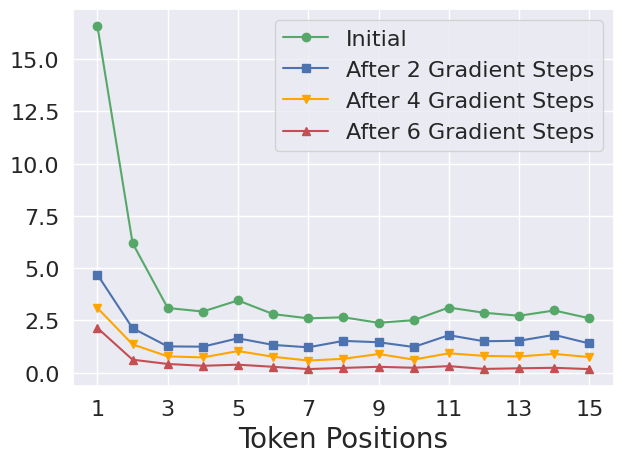
\includegraphics[width=\textwidth]{figs/pure_bad_token_wise_plot/loss.png}
      \caption{Per-token Cross-Entropy Loss\\ on The Fine-tuning Dataset}
      \label{fig:pure_bad_loss}
  \end{subfigure}
  \hfill
  \centering
  \begin{subfigure}{0.32\textwidth}
      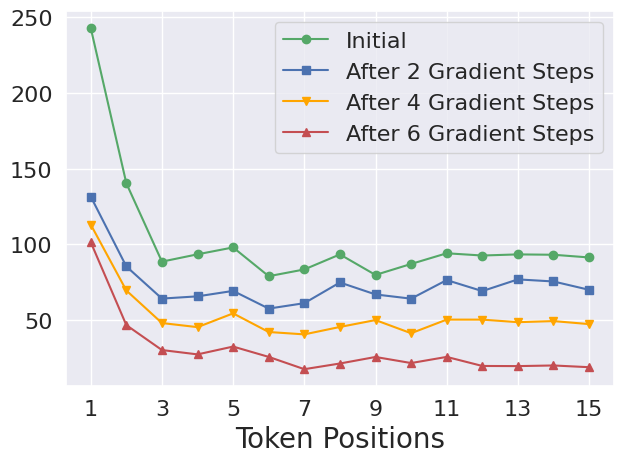
\includegraphics[width=\textwidth]{figs/pure_bad_token_wise_plot/gradient_norm.png}
       \caption{Per-token Gradient Norm\\on The Fine-tuning Dataset}
       \label{fig:pure_bad_gradient}
   \end{subfigure}
  \hfill
  \begin{subfigure}{0.32\textwidth}
      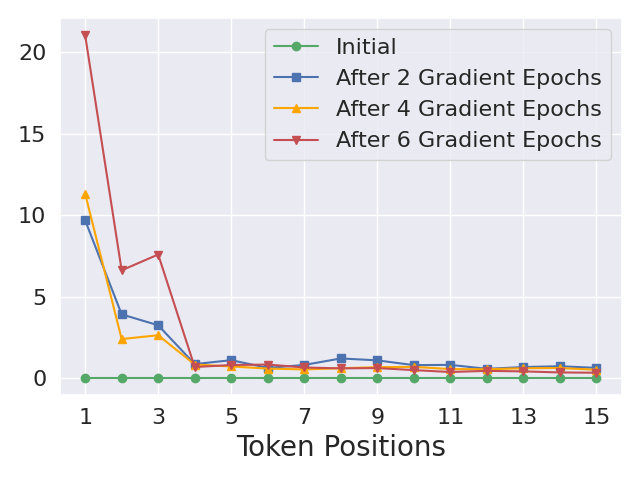
\includegraphics[width=\textwidth]{figs/pure_bad_token_wise_plot/kl_divergence.png}
      \caption{Per-token KL Divergence on\\HEx-PHI Safety Test Dataset~\cite{hexphi}}
      \label{fig:pure_bad_kl}
  \end{subfigure}
  \caption{Then per-token dynamics when fine-tuning Llama-2-7B-Chat on the 100 Harmful Examples from \citet{qi2023fine}. \textit{Note: 1) ASR of initially aligned model = \underline{1.5\%}; 2) After 2 gradient steps = \underline{22.4\%}; 3) After 4 gradient steps = \underline{76.4\%}; 4) After 6 gradient steps = \underline{87.9\%}.}}
  \label{fig:pure_bad_per_token_dynamics}

  \end{figure}


%The safety shortcut perspective that we underscore in Section~\ref{sec:shallow_alignment} provides us with a straightforward view of why the current safety alignment can be so easily removed via fine-tuning. At the high level, if the primary effect of safety alignment concentrates on adjusting the generative distribution of only the first few tokens of refusal prefixes, then breaking it is also just a matter of unlearning such prefixes. To validate this argument, we take the same 100 (harmful instruction, harmful answer) data pairs that \citet{qi2023fine} used for fine-tuning attacking and examine how the fine-tuning on these data points impacts the generative distribution of an aligned model at a per-token level.





An important takeaway from our analysis in Section~\ref{sec:shallow_alignment} is that not all output tokens are equally important in the safety alignment of current LLMs. %Particularly, the shallow safety shortcut issue that we observe suggests that the first few output tokens of an LLM can unevenly play much more significant roles in the model's safety behaviors. 
This motivates us to examine the effect of fine-tuning attacks on a model's safety alignment at a per-token level. 

Formally, the standard custom fine-tuning of an aligned LLM on a dataset $D$ is characterized by the following optimization loss function, where $\pi_{\theta}$ is initialized with the aligned model $\pi_{aligned}$:
\begin{align}
    & \min_{\theta} \Bigg\{\ \mathop{\mathbb E}_{(\bx,\by)\sim D}  - \log \pi_{\theta}\big[\by|\bx\big] \ \Bigg\} \ \ = \ \  \min_{\theta} \Bigg\{\ \ \mathop{\mathbb E}_{(\bx,\by)\sim D}  - \sum_{t=1}^{|\by|} \log \pi_{\theta}\big[y_t|\bx, y_1, ..., y_{t-1}\big]\ \ \Bigg\}
\label{eqn:sft}
\end{align}
%On each data point $(\bx, \by)$, we can decompose the objective into a sum of per-token loss values $-\log \pi_{\theta}\big[\by_t|\bx, \by_1, ..., \by_{t-1}\big]$ for the output token $\by_t$ at each position $t$. Therefore, it is feasible to 
We investigate the per-token dynamics of the fine-tuning process by separately examining:
\begin{enumerate}
    \item The per-token cross-entropy loss at each token position $t$: $-\log \pi_{\theta}\big[y_t|\bx, y_1, ..., y_{t-1}\big]$ 
    \item The gradient magnitude of the per-token loss: $\big\|-\nabla \log \pi_{\theta}\big[y_t|\bx, y_1, ..., y_{t-1}\big]\big\|_2$
\end{enumerate}


We also examine the per-token KL divergence between the fine-tuned models' generative distribution and that of the initially aligned model on the harmful instructions from the HEx-PHI safety test benchmark~\cite{hexphi}. Specifically, for a harmful instruction $\tilde \bx$, we take the outputs $\tilde \by \sim \pi_{\theta}[\cdot | \tilde\bx ]$ from the fine-tuned model $\pi_{\theta}$. Then, for each token position $t$, we compute the KL divergence $KL\big[\pi_{\theta}(\cdot | \tilde\bx, \tilde y_1, ..., \tilde y_{t-1}) \big\| \pi_{aligned} (\cdot | \tilde\bx, \tilde y_1, ..., \tilde y_{t-1})\big]$. 

Figure~\ref{fig:pure_bad_per_token_dynamics} presents such a per-token decoupling of the harmful example demonstration attack from \citet{qi2023fine}. Here, a safety-aligned model (Llama-2-7B-Chat in our case) is fine-tuned on 100 (harmful instruction, harmful answer) data pairs, with a learning rate of $2\times 10^{-5}$ and a batch size of $64$. Figure~\ref{fig:pure_bad_loss} shows the average per-token loss on the 100 data points, Figure~\ref{fig:pure_bad_gradient} plots the average gradient magnitude induced by the per-token loss, and Figure~\ref{fig:pure_bad_kl} illustrates the per-token KL divergence between the fine-tuned models and the initially aligned model.

We note that \textbf{the token-wise decoupling clearly exposes an uneven impact of the fine-tuning attack across token positions.} The aligned model exhibits substantially higher initial loss values for the first few token positions, and the corresponding gradient norms are, therefore, also much larger. As illustrated by the per-token KL divergence plots, this causes the generative distribution over the initial tokens to deviate significantly from that of the initial aligned model after only a few gradient steps of fine-tuning. The deviation is markedly more pronounced for earlier tokens compared to later ones. Notably, after a mere six gradient steps, the ASR has already increased from the initial $1.5\%$ to $87.9\%$. These per-token dynamics symmetrically echo our observations in Section~\ref{sec:shallow_alignment}. On the one hand, the shallow safety alignment issue infers that the safety alignment of current models is predominantly biased toward the generative distribution of the initial refusal tokens. Conversely, the per-token dynamics of the fine-tuning attacks suggest that the poor durability of the safety alignment essentially also results from the ease of unlearning the distribution of these safety-critical initial tokens --- the large gradient norms (Figure~\ref{fig:pure_bad_gradient}) for the early tokens readily lead to rapid divergence of their generative distribution (Figure~\ref{fig:pure_bad_kl}).


\begin{wrapfigure}{l}{0.41\textwidth}
\vspace{-2.0em}
\begin{center}
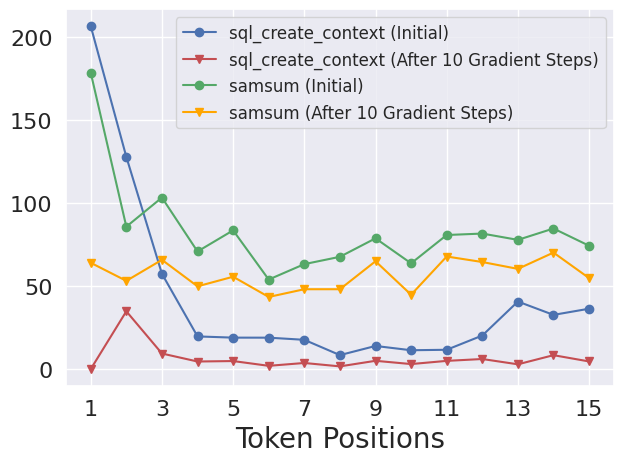
\includegraphics[width=\linewidth]{figs/benign_gradient.png}
\end{center}
\vspace{-1em}
\caption{Per-token Gradient Norm When Fine-tuning Llama-2-7B-Chat on Benign Downstream Tasks Datasets. \textit{Note: 1) ASR of initially aligned model = \underline{$1.5\%$}; 2) After 10 gradient steps on SQL Create Context} = \underline{$13.6\%$}; 3) After 10 gradient steps on Samsum = \underline{$22.1\%$}.}
\vspace{-1em}
\label{fig:benign_gradient}
\end{wrapfigure} 

Interestingly, in addition to fine-tuning attacks where the fine-tuning datasets are intentionally designed to be harmful, \textbf{we also note similar per-token dynamics even on purely benign downstream fine-tuning cases.} Specifically, Figure~\ref{fig:benign_gradient} plots the gradient norm when fine-tuning Llama-2-7B-Chat on SQL Create Context~\cite{b-mc2_2023_sql-create-context} and Samsum~\cite{samsum}. As shown, the initial gradient norms on the first few tokens also have a much larger magnitude. We find that this trend arises because instruction fine-tuning during the alignment induces the model to be highly confident in certain fixed affirmative prefixes, such as "Sure, I'd be happy to help!" on normal inputs. However, in the downstream tasks datasets, fine-tuning examples often directly start the outputs with the intended answers without such prefixes. Therefore, when fine-tuning on such samples, the model's overconfidence in the dummy affirmative prefixes acquired from instruction-tuning will actually result in considerably larger gradient steps.



We hypothesize that 
\prateek{why are we speculating instead of confirming all this?}
\ashwinee{prateek, how do you think we can ``confirm'' something? it would be far too strong of a statement to say that ``we show that...''}
\textbf{this might be one underlying reason why \citet{qi2023fine} discover that even benign fine-tuning can cause safety regression in the aligned LLMs} --- it may merely result from the excessively larger gradient steps when unlearning the generative distributions of these initial dummy tokens, which, in turn, lead to over-generalization~(or catastrophic forgetting), and therefore unintendedly also disrupt the model's generative distribution for refusal prefixes conditioned on harmful inputs. This is plausible, as we note that a full fine-tuning on SQL Create Context and Samsum with more than 600 gradient steps results in an increase of ASR from $1.5\%$ to 14.9\% and 25.5\% respectively, but the ASR is already at 13.6\% and 22.1\% after the initial 10 gradient steps on the two datasets. This suggests that the most significant safety regression exactly occurs during these early steps when the gradient norm for the initial tokens is excessively large.
\end{comment}























\subsection{Safer Custom Fine-tuning via Token-wise Regularization}
\label{subsec:fine-tuning-regularization}

The per-token dynamics in Section~\ref{subsec:fine-tuning-analysis} suggest that the safety failure after follow-up fine-tuning could be largely attributed to the distribution shift at only the first few tokens. Although this presents another frustrating view of the shallowness of the safety alignment, we note that it also implies a potential avenue for mitigation! Specifically, we posit that:
\begin{quote}
\textit{If the very first few output tokens play such a 
decisive role in a model's safety alignment, then we should be able to protect the alignment from being compromised by simply imposing constraints to ensure that the generative distribution of these initial tokens does not significantly deviate from the original state.}
\end{quote}



This motivates us to devise the following regularized fine-tuning objective as opposed to the standard cross-entropy objective in Eqn~\ref{eqn:sft}:
\begin{align}
    & \min_{\theta} \Bigg\{ \ \ \mathop{\mathbb E}_{(\bx,\by)\sim D} -  \sum_{t=1}^{|\by|} \frac{1}{\beta} \log\Bigg[\sigma \bigg( \beta \cdot  \log \frac{\pi_{\theta}\big[y_t|\bx, y_1,...,y_{t-1}\big]}{\pi_{aligned}\big[y_t|\bx, y_1,...,y_{t-1}\big]}  \bigg)  \Bigg] \ \ \Bigg\}
\label{eqn:soft-sft-uniform}
\end{align}
Here, $\sigma(\cdot)$ is the sigmoid function and $\beta$ is a constant parameter that controls the speed of the saturation of the sigmoid. The gradient of this objective on a data point $(\bx, \by)$ is derived as:
\begin{align}
    &  -  \sum_{t=1}^{|\by|} w_t \times \nabla \ \log \ \pi_{\theta}\big[y_t|\bx, y_1,...,y_{t-1}\big],\ w_t := \Bigg[1 - \sigma\Bigg( \beta \cdot \log \frac{\pi_{\theta}\big[y_t|\bx, y_1,...,y_{t-1}\big]}{\pi_{aligned}\big[y_t|\bx, y_1,...,y_{t-1}\big]}\Bigg)\Bigg]
\end{align}
Note that, the gradient of the cross-entropy loss in Eqn~\ref{eqn:sft} is $-  \sum_{t=1}^{|\by|}  \nabla \ \log \ \pi_{\theta}\big[y_t|\bx, y_1,...,y_{t-1}\big]$. Therefore, in comparison, the new loss function in Eqn~\ref{eqn:soft-sft-uniform} essentially just applies an additional adaptive weight $w_t$ for the token-wise gradient term of the original objective. The weight $w_t$ will decrease when the log ratio inside $\sigma(\cdot)$ function is large. It is easy to see that this log ratio essentially characterizes the deviation between the fine-tuned model $\pi_{\theta}$ and the initially aligned model $\pi_{aligned}$ at the token position $t$. Taking together, we can see that the fine-tuning objective will adaptively diminish the weight of those token positions where the deviation of the distribution approaches a certain threshold (controlled by $\beta$), thereby constraining it from further deviation. In Appendix~\ref{appendix:derivation_of_loss_regularization}, we also show how this loss function can also be derived from a reinforcement learning optimization objective with KL divergence constraint.

We have noted the unevenly more significant role that the first few tokens play in a model's safety. Therefore, in implementation, we also find it beneficial to set generally larger $\beta$ for the first few tokens. The larger $\beta$ will make the weight $w_t$ diminish faster and, therefore, represents a stronger constraint on the deviation of the generative distribution on these tokens. This finally leads to the following implementation: 
\begin{align}
    \label{eqn:soft-sft-biased}
    & \min_{\theta} \Bigg\{ \ \ \mathop{\mathbb E}_{(\bx,\by)\sim D} -  \sum_{t=1}^{|\by|} \frac{1}{\beta(t)} \log\Bigg[\sigma \bigg( \beta(t) \cdot  \log \frac{\pi_{\theta}\big[y_t|\bx, y_1,...,y_{t-1}\big]}{\pi_{aligned}\big[y_t|\bx, y_1,...,y_{t-1}\big]}  \bigg)  \Bigg] \ \ \Bigg\}, \ \beta(t) = 
    \begin{cases} 0.5 , & t =1 \\
        2.0 & 2 < t <= 5 \\
        0.1 , & \text{otherwise}
    \end{cases}
\end{align}




%\xiangyu{I tried adding lucy's attack here, but it does not work for learning rate = $2\times 10^{-5}$.}

\begin{table}[!htbp]
\caption{Main Table}
\centering
  \resizebox{.9\linewidth}{!}{

\begin{tabular}{c|c|c|c|c|c|c|c|c}
\hline
\multicolumn{2}{c|}{Models $\rightarrow$} &  \multicolumn{3}{c|}{Llama-2-7B-Chat} & & \multicolumn{3}{c}{Gemma-1.1-7B-IT}\\
\hline
\multirow{2}*{\shortstack{Datasets $\downarrow$}} & & \multirow{2}*{\shortstack{Initial}} & \multirow{2}*{\shortstack{Standard\\SFT}} & \multirow{2}*{\shortstack{\textbf{Constrained}\\\textbf{SFT (ours)}}} & & \multirow{2}*{\shortstack{Initial}} & \multirow{2}*{\shortstack{Standard\\SFT}} & \multirow{2}*{\shortstack{\textbf{Constrained}\\\textbf{SFT (ours)}}} \\ 
&   &  &  &  &   &  & &\\
\hline
\multicolumn{9}{c}{\textit{Against Fine-tuning Attacks}}\\
\hline
Harmful Examples & ASR   &  1.5\%  &  88.9\%  &  4.6\%  & &  1.8\% &  81.6\% & 1.9\% \\
\hline
Identity Shifting & ASR   &  0\% & 
 79.5\%   &   8.1\% & &  0\% &  83.6\% & 9.1\% \\
%\hline
%Data Selection~\citep{he2024s} &  ASR  & 3.6\%  &    &    &    &  \\
\hline
\multirow{2}*{\shortstack{Backdoor\\Poisoning}}  & ASR (w/o trigger)   & 1.5\%   & 7.6\%   &  1.9\% & &  1.8\% &  2.0\% & 1.5\% \\
 & ASR (w/ trigger)  &  1.7\%  & 90.9\%   & 10.9\%  & & 1.8\%  &  82.3\% & 1.9\% \\
\hline
\multicolumn{9}{c}{\textit{Fine-tuning with Normal Downstream Datasets}}\\
\hline
\multirow{2}*{\shortstack{Samsum}} & ASR  & 1.5\% &   23.4\%  &   3.2\%  & &  1.8\% &  2.0\% & 2.4\% \\
&  Utility & 25.5\% & 51.7\%  &   50.1\%  & &  36.0\% &  51.5\% & 51.9\% \\
\hline
\multirow{2}*{\shortstack{SQL Create Context}} & ASR  & 1.5\%  & 15.4\%  & 3.2\%   & &  1.8\% &  2.8\% & 2.4\% \\
&  Utility & 14.9\% & 99.1\%  &  98.5\%  & &  88.0\% &  99.2\% & 98.6\% \\
\hline
\multirow{2}*{\shortstack{GSM8k}} & ASR  & 1.5\% & 3.3\% &   2.0\%  & &  1.8\% &  2.9\% & 1.7\% \\
&  Utility & tbd & 41.7\% &  37.4\% & &  tbd &  63.3\% & 63.6\% \\
\hline
\end{tabular}}
\label{tab:main}
\end{table}

\xiangyu{todo: summarize results}

\xiangyu{todo: add the log ratio plot to explain why the regularization can let utility datasets go through via suppressing the attacks.}



%Table~\ref{tab:llama-2-finetuning} suggests that both warmup and soft-soft are helpful for better safety performance. Particularly, for warmup:
%\begin{enumerate}
%    \item The warmup is important because the initial gradient norms will be very large, and using a gentle start is generally beneficial to avoid the model's safety being broken by large update steps.
%    \item Soft-soft does not apply a penalty on the early tokens at the start of fine-tuning, while the early gradient steps are large. It's likely that when the penalty starts to apply, safety is already broken. Warmup ensures the sigmoid is smoothly saturated and thus the penalty is smoothly initialized. 
%\end{enumerate}

\begin{comment}
\begin{table}[!htbp]
\caption{Fine-tuning Llama-2-7b-Chat (deprecated)}
\centering
  \resizebox{.95\linewidth}{!}{

\begin{tabular}{c|c|c|c|c|c|c}
\hline
\multirow{2}*{\shortstack{Datasets}} & & \multirow{2}*{\shortstack{Initial}} & \multirow{2}*{\shortstack{Standard\\SFT}} & \multirow{2}*{\shortstack{Unbiased Regularization\\$\beta = 0.1, \alpha = 0$}} & \multirow{2}*{\shortstack{Unbiased Regularization\\$\beta = 2.0, \alpha = 1.0$}} & \multirow{2}*{\shortstack{Biased Regularization\\$\beta(t), \alpha(t)$ in Eqn~\ref{eqn:soft_sft}}} \\ 
&   &  &  &  &   & \\
\hline
\multirow{2}*{\shortstack{Harmful Examples}}  & ASR   & - & 33.9  &  18.3 & 1.1 & \textbf{1.8} \\
&  Utility & - & -  &  - &  - & - \\
\hline
\multirow{2}*{\shortstack{Identity Shifting (AOA)}} & ASR  & - & 50.6  &  49.4 & 20.6 & \textbf{19.8}   \\
&  Utility & - & -  &  - &  - & -  \\
\hline
\multirow{2}*{\shortstack{Samsum}} & ASR  & - & 6.4  &  4.4 & 1.9 &  1.8   \\
&  Utility & - & 52.0  &  51.8 & 41.6 & 49.8  \\
\hline
\multirow{2}*{\shortstack{SQL Create Context}} & ASR  & - & 2.2  &  2.2 & 2.2 & 1.9   \\
&  Utility & - & 99.1  &  99.0 & 97.6 & 98.4  \\
\hline
\multirow{2}*{\shortstack{GSM8k}} & ASR  & - & 3.1  &  4.7 & 4.2 & 5.5   \\
&  Utility & - & 34.7  &  34.7 & 4.1 & 34.9  \\
\hline
\end{tabular}}
\label{tab:llama-2-finetuning-old}
\end{table}
\end{comment}

\begin{comment}
\begin{table}[!htbp]
\caption{Fine-tuning Gemma-1.1-7b-it}
\centering
  \resizebox{.95\linewidth}{!}{

\begin{tabular}{c|c|c|c|c|c}
\hline
\textbf{Datasets} & & {\textbf{Initial}} & {\textbf{Standard SFT}} & {\textbf{Unbiased Regularization}} & {\textbf{Biased Regularization}} \\
\hline
\multirow{2}*{\shortstack{Harmful Examples}}  & ASR   & - & 92.2  &  - &  \textbf{6.1} \\
&  Utility & - & -  &  - &  - \\
\hline
\multirow{2}*{\shortstack{Identity Shifting (AOA)}} & ASR  & - & 62.5  &  - &  \textbf{31.1}   \\
&  Utility & - & -  &  - &  -  \\
\hline
\multirow{2}*{\shortstack{Samsum}} & ASR  & - & 12.8  &  - &  12.7   \\
&  Utility & - & 51.7  &  - &  48.1  \\
\hline
\multirow{2}*{\shortstack{SQL Create Context}} & ASR  & - & 2.5  &  - &  2.0   \\
&  Utility & - & 99.1  &  - &  97.5  \\
\hline
\multirow{2}*{\shortstack{GSM8k}} & ASR  & - & 3.1  &  - &  3.5   \\
&  Utility & - & 61.7  &  - &  61.3  \\
\hline
\end{tabular}}
\label{tab:llama-2-finetuning}
\end{table}

\begin{table}[!htbp]
\caption{Fine-tuning Mistral-7b-Instruct-v0.2 \ashwinee{WIP}}
\centering
  \resizebox{.95\linewidth}{!}{

\begin{tabular}{c|c|c|c|c|c}
\hline
\textbf{Datasets} & & {\textbf{Initial}} & {\textbf{Standard SFT}} & {\textbf{Unbiased Regularization}} & {\textbf{Biased Regularization}} \\
\hline
\multirow{2}*{\shortstack{Harmful Examples}}  & ASR   & - & 90.41&  - &  0\\
&  Utility & - & -  &  - &  - \\
\hline
\multirow{2}*{\shortstack{Identity Shifting (AOA)}} & ASR  & - & &  - &  \\
&  Utility & - & -  &  - &  -  \\
\hline
\multirow{2}*{\shortstack{Samsum}} & ASR  & - & &  - &  \\
&  Utility & - & &  - &  \\
\hline
\multirow{2}*{\shortstack{SQL Create Context}} & ASR  & - & &  - &  \\
&  Utility & - & &  - &  \\
\hline
\multirow{2}*{\shortstack{GSM8k}} & ASR  & 8.61& 30.83&  - &  21.66\\
&  Utility & - & 51.93&  - &  52.38\\
\hline
\end{tabular}}
\label{tab:mistral-finetuning}
\end{table}

\begin{table}[!htbp]
\caption{Fine-tuning LLaMA-3-8B-Instruct \ashwinee{WIP}}
\centering
  \resizebox{.95\linewidth}{!}{

\begin{tabular}{c|c|c|c|c|c}
\hline
\textbf{Datasets} & & {\textbf{Initial}} & {\textbf{Standard SFT}} & {\textbf{Unbiased Regularization}} & {\textbf{Biased Regularization}} \\
\hline
\multirow{2}*{\shortstack{Harmful Examples}}  & ASR   & - & 84.16&  - &  85.83\\
&  Utility & - & -  &  - &  - \\
\hline
\multirow{2}*{\shortstack{Identity Shifting (AOA)}} & ASR  & - & &  - &  \\
&  Utility & - & -  &  - &  -  \\
\hline
\multirow{2}*{\shortstack{Samsum}} & ASR  & - & &  - &  \\
&  Utility & - & &  - &  \\
\hline
\multirow{2}*{\shortstack{SQL Create Context}} & ASR  & - & &  - &  \\
&  Utility & - & &  - &  \\
\hline
\multirow{2}*{\shortstack{GSM8k}} & ASR  & & 3.88&  - &  \\
&  Utility & - & 72.17&  - &  \\
\hline
\end{tabular}}
\label{tab:llama3-finetuning}
\end{table}
\end{comment}

